\documentclass{mcmthesis}
\mcmsetup{CTeX =false,   % 使用 CTeX 套装时,设置为 true
        , problem = 8,
        sheet = true, titleinsheet =true, keywordsinsheet = true,
        titlepage =false, abstract = false}
\usepackage{palatino}
\usepackage{lipsum}

\usepackage{geometry}
%===============设置正文和数学字体=============================
%有些字体需要安装一些字体文件,注意辨别。
%我参照 MCM论文集的字体 使用如下宏包来定制字体。
%%%%%%%%%%%%%%%%%%%%%%%%%%%%%%%%%%%%%%%%%%%%%%%%
%lhr的包
\usepackage{graphicx}
%\graphicspath{ {./images/} }
\usepackage{float} 
\documentclass{article}
\usepackage[utf8]{inputenc}
\usepackage{booktabs} %三线表需要加载宏包{booktabs}
\usepackage{diagbox}
\usepackage{multirow}
\usepackage{listings}
\usepackage{xcolor}
\usepackage{clrscode3e}
\usepackage{algorithm}  
\usepackage{algpseudocode}  
\usepackage{amsmath}  
\renewcommand{\algorithmicrequire}{\textbf{Input:}}  % Use Input in the format of Algorithm  
\renewcommand{\algorithmicensure}{\textbf{Output:}} % Use Output in the format of Algorithm 
\makeatletter
\newif\if@restonecol
\makeatother
\let\algorithm\relax
\let\endalgorithm\relax
\usepackage[linesnumbered,ruled,vlined]{algorithm2e}%[ruled,vlined]{
\usepackage{algpseudocode}
\usepackage{amsmath}
\renewcommand{\algorithmicrequire}{\textbf{Input:}}  % Use Input in the format of Algorithm
\renewcommand{\algorithmicensure}{\textbf{Output:}} % Use Output in the format of Algorithm

%子图的包
\usepackage{graphicx}
\usepackage{subfigure}

%表格的包
\usepackage[utf8]{inputenc}
\usepackage{booktabs} %三线表需要加载宏包{booktabs}
\usepackage{diagbox}
\usepackage{multirow}
\usepackage{listings}
\usepackage{xcolor}

%New colors defined below
\definecolor{codegreen}{rgb}{0,0.6,0}
\definecolor{codegray}{rgb}{0.5,0.5,0.5}
\definecolor{codepurple}{rgb}{0.58,0,0.82}
\definecolor{backcolour}{rgb}{0.95,0.95,0.92}

%Code listing style named "mystyle"
\lstdefinestyle{mystyle}{
  backgroundcolor=\color{backcolour},   commentstyle=\color{codegreen},
  keywordstyle=\color{magenta},
  numberstyle=\tiny\color{codegray},
  stringstyle=\color{codepurple},
  basicstyle=\ttfamily\footnotesize,
  breakatwhitespace=false,         
  breaklines=true,                 
  captionpos=b,                    
  keepspaces=true,                 
  numbers=left,                    
  numbersep=5pt,                  
  showspaces=false,                
  showstringspaces=false,
  showtabs=false,                  
  tabsize=2
}

%"mystyle" code listing set
\lstset{style=mystyle}
%%%%%%%%%%%%%%%%%%%%%%%%%%%%%%%%%%%%%%%%%%%%%%%%%%
\usepackage{graphicx}
\usepackage{subfigure}
%设置段落之间的距离,若不需要删除或者注释掉即可。
\setlength\parskip{.5\baselineskip}
\newtheorem{definition}{Definition}[section]
%\def\abstractname{Summary}%可修改摘要名称

\usepackage{indentfirst}
\setlength{\parindent}{2em}

\usepackage{chngpage}
\usepackage{array}
\usepackage{booktabs}
\usepackage{threeparttable}
\usepackage{longtable}
\usepackage[numbers,sort&compress]{natbib}
%%% 实现参考文献标号在右上角
\newcommand{\upcite}[1]{\textsuperscript{\textsuperscript{\cite{#1}}}}
%然后引用的时候使用\upcite{}的格式(一般的正常引用格式为\cite{})

\usepackage{titletoc}
\titlecontents{section}[3cm]{\bf \large}{\contentslabel{2.8em}}{}{%
\titlerule*[0.5pc]{$\cdot$}\contentspage}%
\titlecontents{subsection}[4cm]{\normalsize}{\contentslabel{2.5em}}{}{%
\titlerule*[0.5pc]{$\cdot$}\contentspage}%
\titlecontents{subsubsection}[5.3cm]{\normalsize}{\contentslabel{3.0em}}{}{%
\titlerule*[0.5pc]{$\cdot$}\contentspage}%

\title{\large Optimal Control of a Linear Discrete System}

\author{Dazheng Fang//Haorui li//Yao Yao//Zhiyi Shi }


\date{\today}

\geometry{left=3.0cm,right=3.0cm}

\begin{document}


\begin{abstract}

In the real world, many real systems are time-discrete in nature.Even if the system is time-continuous, because the computer is based on such discrete digital technology as time and value, the implementation of computer control must be treated as a discrete system after time discrimination.Therefore, it is necessary to discuss the optimal control of discrete time systems.

To build up the optimal problem, first, we define the objective function in chapter-3 which stands for summation of the magnitude square of controls over the entire time horizon.And we want to constrain the x(T) to fall in the predetermined interval, so a penalty function is defined in chapter-4. If the L increases which means the final state x(T) will have a greater impact on the objective function, therefore x(T) would have a much stricter constrains and this would cause the decrease of the final state value. Vice versa, if the L reduces, the value of x(T) would be larger
Therefore, by changing the value of coefficient L we are able to control the X(T) to fall in the interval that we wanted.

We have used lots of methods to solve the problem in the matlab. But finally, only interior point method can match our problem. We write our own function and use interior point method to optimize it. For the problems that need to be solved, we adjusted the parameters and measured multiple sets of data. We reached a detailed conclusion, which will be introduced in detail in our article.

%求解问题

%%%%%%%%%%%%%%%%%%%%%%%%%%%%%%%%%%%%%%%%%%%%%%

\begin{keywords}
DLQR; Interior point method;  Dynamic programming; MATLAB; \\\\\\
Author: Dazheng Fang , Haorui Li, Yao Yao, Zhiyi Shi (Alphabetical order)
\end{keywords}


\end{abstract}
\maketitle
%\pagestyle{empty}
\newpage                                                          %
%==================================================================
%====================生=成=目=录===================================
\begin{adjustwidth}{-1cm}{0cm}

\setcounter{tocdepth}{3}
\thispagestyle{empty}
\tableofcontents                                                  %

\end{adjustwidth}


\newpage

\pagestyle{fancy}

\setcounter{page}{1}
\section{Introduction}
\subsection{Background}

In the real world, many real systems are time-discrete in nature.Even if the system is time-continuous, because the computer is based on such discrete digital technology as time and value, the implementation of computer control must be treated as a discrete system after time discretization.\cite{journals/kybernetika/StechaKKL73}

Therefore, it is necessary to discuss the optimal control of discrete time systems.


\subsection{Problem Restatement}

Suppose that we have a discrete-time linear system with the following dynamic equation:

$$\begin{array}{l}
x(k+1)=A x(k)+B u(k) \\
\end{array}$$

where x(t) is the state variable at time t; u(t) is control variable at time t; A is the state matrix; and B is the control matrix. Suppose that the initial state x(0) is known. Demine the control series u(t), t=0, 1, …, T, such that the state at the end of the time horizon x(T) falls in a predetermined interval and the energy consumed in the entire time horizon (which can be captured by the weighted summation of the magnitude square of controls over time) can be minimized. The values of the controls have upper bounds.

And the six problems are:

(1)	Develop the mathematical programming model of the optimal control problem.

(2)	Set up the scale of the problem (i.e., the dimension of the state vector and the control vector) by yourself, as well as the values of the matrices A and B, the initial state and the upper bounds of the controls. Solve the problem by using the tools in Matlab and obtain the optimal control policy.

(3)	Change the value of A and analyze its impact on the controls and the objective function.

(4)	Change the upper bounds of the controls and analyze their impact on the controls and the objective function.

(5)	Change the length of the time horizon (i.e., the value of T) and analyze its impact on the controls and the objective function.

(6)	Write a research report, which must include the description of the problem, definition of the notations, explanation of the data, mathematical formulation of the problem, method of solving the problem, analysis of the result, conclusion, and references. The source code must be submitted.


\subsection{Our Work}
First of all, we define the objective function and add a penalty function to build up the optimal problem. Then we tried DLQR, simulink, dynamic programming and interior point method to solve the problem. Finally we change the parameters like A, B, and T to track their influences on results.


\section{List of Notation}

\begin{center}
\begin{longtable}{p{.1\textwidth}p{.8\textwidth}m{.4\textwidth}}
\caption{The List of Notation}\\
\hline
Symbol& Meaning \\
\hline

$J$      & System performance index, optimization function
                                                         \\
$\bar J$ & Cost function    \\
$L_k$      & The increment of performance indicator J in the Kth sampling period
                                                          \\
$\lambda$     & Lagrangian multiplier matrix\\
$L$     & Penalty weight for x
                                                                                        \\ \hline

 \end{longtable}
 \end{center}


\section{Problem One: Build up the Model}
From the problem we define the system performance index, in other words, optimization function J as:
%%%%%%%%%要不要加权?%%%%%%%%%%
$$J=\frac{1}{2}\sum^{T-1}_{k=0}u^T(k)u(k)+Lx(T)^Tx(T)$$
\\  We define the objective function as above. The first term stands for summation of the magnitude square of controls over the entire time horizon which also means the energy consumed by the whole system. However, if we want to constrain the x(T) to fall in the predetermined interval, a penalty function should be defined like the second term. If the L increases which means the final state x(T) will have a greater impact on the objective function, therefore x(T) would have a much stricter constrains and this would cause the decrease of the final state value. Vice versa, if the L reduces, the value of x(T) would be larger.
Therefore, by changing the value of coefficient L we are able to control the X(T) to fall in the interval that we wanted.\\
$Notes$ : Now the weight of every step is 1

The problem can be rewriten as:
\begin{align}
min & \text{ } J=\frac{1}{2}\sum^{T-1}_{k=0}u^T(k)u(k)+Lx^T(T)x(T)\\
S.t. \text{ }& x(k+1)=A x(k)+B u(k)\\ &  k < T\\& k \in Z^+ \\&x(0)=x_0\\&u(k)\leq U
\end{align}


\section{Problem Two: Solve the problem by using thetools in Matlab }
We search different MATLAB tools and finally tried the following methods:

\begin{itemize}

\item QLDR Function
\item Interior Point Method
\item Dynamic Programming 
\item Euler Equation

\end{itemize}

Finally the QLDR and interior point method get the best results, due to the time limit, we give up DP and Euler Equation.

\subsection{DLQR Function}

The linear quadratic regulator (LQR) is a well-known design technique that provides practical feedback gains.\cite{journals/corr/WangMD14}\cite{conf/iros/AmesK19}

In the case of the Linear Quadratic Regulator (with zero terminal cost), we can get:

$$L=\frac{1}{2} x^{T} Q x+\frac{1}{2} u^{T} R u$$

where the requirement that L > 0 implies that both Q and R are positive definite. In the
case of linear plant dynamics also, we have


$$\begin{aligned}
&L_{x} =x^{T} Q \\
&L_{u} =u^{T} R \\
&f_{x} =A \\
&f_{u} =B
\end{aligned}$$

So we have:

$$\begin{aligned}
&\dot{x} =A x+B u \\
&x\left(t_{o}\right) =x_{o} \\
&\dot{\lambda}=-Q x-A^{T} \lambda  \\
&\lambda\left(t_{f}\right) =0 \\
&R u+B^{T} \lambda =0
\end{aligned}$$

Since the systems are clearly linear, we try a connection λ = Px. Inserting this into the η˙
equation, and then using the $\dot{x}$˙ equation, and a substitution for u, we obtain:

$$P A x+A^{T} P x+Q x-P B R^{-1} B^{T} P x+\dot{P}=0$$

This has to hold for all x, so in fact it is a matrix equation, the matrix Riccati equation.
The steady-state solution is given satisfies:
$$P A+A^{T} P+Q-P B R^{-1} B^{T} P=0$$

This equation is the matrix algebraic Riccati equation (MARE), whose solution P is needed
to compute the optimal feedback gain K. The MARE is easily solved by standard numerical
tools in linear algebra.
The equation $Ru + B^T \lambda$ = 0 gives the feedback law:

$$u = −R^{−1}B^{T}Px$$

The LQR generates a static gain matrix K, which is not a dynamical system.\cite{conf/rait/BhushanCS16}
Hence, the order of the closed-loop system is the same as that of the plant.
\subsection{Use LQR in MATLAB}
Under the derivation of the LQR, we can write the following code in order to obtain the static gain matrix K. Simultaneously, we can draw the output of the system over time where we can see clearly that the system approaching a stable value.

\begin{lstlisting}[language=MATLAB, caption=LQR in MATLAB]
A=[0 1 0;0 0 1;-35 -27 -9];
B=[0;0;1];
C=[1 0 0 ;0 1 0 ;0 0 1 ];
D=[0;0;0;];
Q=[0 0 0;0 0 0;0 0 0];
R=1;
K=dlqr(A,B,Q,R)
Ac=[(A-B*K)];
Bc=[B];
Cc=[C];
Dc=[D];
t=0:0.005:200;
U=ones(size(t));
x0=[0.05 0.08 0];
[Y,X]=lsim(Ac,Bc,Cc,Dc,U,t,x0);
plot(t,Y);
xlabel('t');
ylabel('Y');
u=-K*X';
\end{lstlisting}

The stable system solved by LQR is as follow:

\begin{figure}[H]%H为当前位置,!htb为忽略美学标准,htbp为浮动图形
  \centering
  \caption{Stable System Solved by LQR}
%可选参数中width=\columnwidth选取了当前列宽
  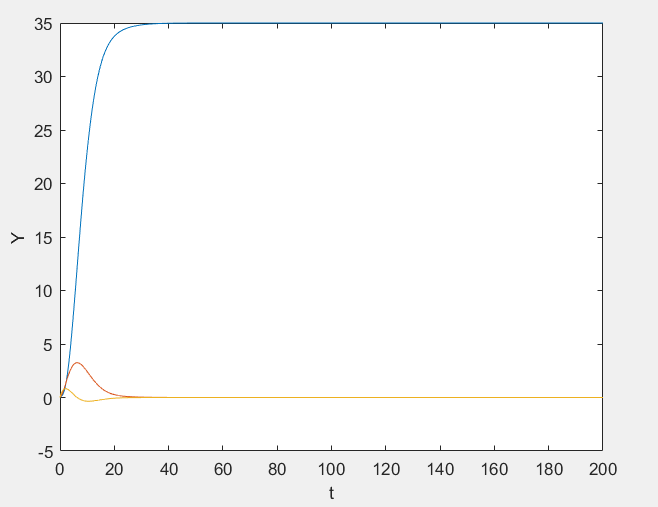
\includegraphics[width=50ex]{Optimal Control of a Linear Discrete System/MCM20200128/picture/LQR结果.png} %插入图片,[]中设置图片大小,{}中是图片文件名
  \label{Fig.RNN} %用于文内引用的标签
\end{figure}
The k it get is:
\begin{figure}[H]%H为当前位置,!htb为忽略美学标准,htbp为浮动图形
  \centering
  \caption{Stable System Solved by LQR}
%可选参数中width=\columnwidth选取了当前列宽
  \includegraphics[width=50ex]{Optimal Control of a Linear Discrete System/MCM20200128/picture/LQRK值.png} %插入图片,[]中设置图片大小,{}中是图片文件名
  \label{Fig.RNN} %用于文内引用的标签
\end{figure}
According to the result of LQR, We can draw the system block diagram of the problem by using Simulink in Matlab. There are totally three blocks in the whole diagram: Discrete State-Space, Gain, Scope.

By applying Discrete State-Space block, with inputting un we can easily obtain yn which in this case is also equivalent to xn+1 as an output. According to the code, we are able to acquire the value of gain K which is mentioned in the LQR. Then we can obtain the negative feedback of the Discrete State-Space block which is -Ky(n). After connecting a scope with the output y(n), we are able to observe the system easily.
\begin{figure}[H]%H为当前位置,!htb为忽略美学标准,htbp为浮动图形
  \centering
  \caption{System in Simulink}
%可选参数中width=\columnwidth选取了当前列宽
  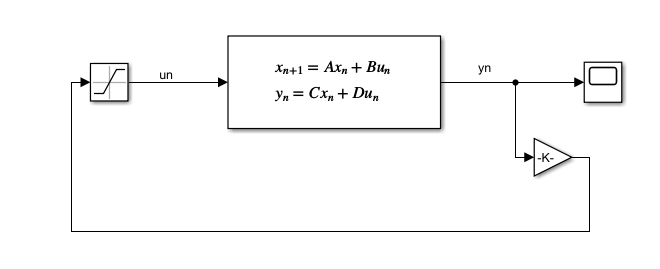
\includegraphics[width=50ex]{Optimal Control of a Linear Discrete System/MCM20200128/picture/框图.png} %插入图片,[]中设置图片大小,{}中是图片文件名
  \label{Fig.RNN} %用于文内引用的标签
\end{figure}
With Simulink we get the oscillogram:
\begin{figure}[H]%H为当前位置,!htb为忽略美学标准,htbp为浮动图形
  \centering
  \caption{System in Simulink}
%可选参数中width=\columnwidth选取了当前列宽
  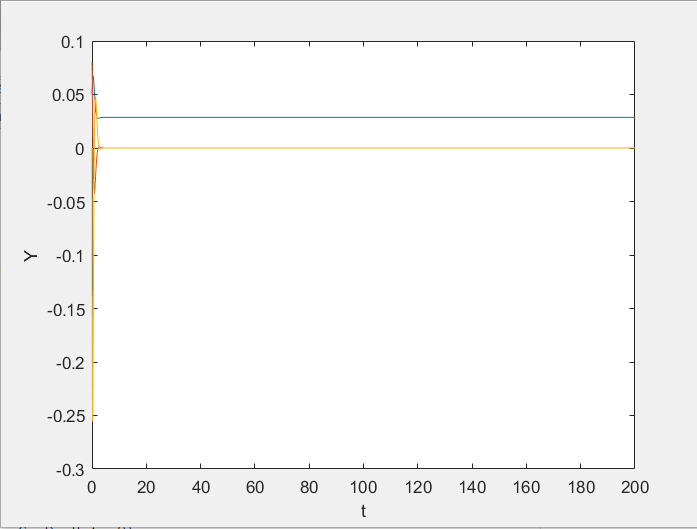
\includegraphics[width=50ex]{Optimal Control of a Linear Discrete System/MCM20200128/picture/波形.png} %插入图片,[]中设置图片大小,{}中是图片文件名
  \label{Fig.RNN} %用于文内引用的标签
\end{figure}

\subsection{Interior Point Method}
We compare the GA\cite{GenTut} tool and the interior point method\cite{conf/aaai/MladenovBK17}  tool in MATLAB, and finally use interior point method get best result.\cite{journals/siamjo/HelmbergRVW96}\cite{journals/software/AstfalkLMS92}\cite{journals/mp/WangMP96}  

The primal-dual method's idea is easy to demonstrate for constrained nonlinear optimization. For simplicity, consider the all-inequality version of a nonlinear optimization problem:
$$\text { minimize } f(x) \text { subject to } c_{i}(x) \geq 0 \text { for } i=1, \ldots, m, x \in \mathbb{R}^{n}, \text { where } f: \mathbb{R}^{n} \rightarrow \mathbb{R}, c_{i}: \mathbb{R}^{n} \rightarrow \mathbb{R}$$

The logarithmic barrier function is
$$B(x, \mu)=f(x)-\mu \sum_{i=1}^{m} \log \left(c_{i}(x)\right)$$

The barrier function gradient is
$$g_{b}=g-\mu \sum_{i=1}^{m} \frac{1}{c_{i}(x)} \nabla c_{i}(x)$$

In addition to the original ("primal") variable x, we introduce a Lagrange multiplier inspired dual variable $\lambda$:

$$c_{i}(x) \lambda_{i}=\mu, \forall i=1, \ldots, m$$

So we get an equation for the gradient:
$$g-A^{T} \lambda=0$$
where the matrix A is the Jacobian of the constraints c(x).

Applying Newton's method we get:

$$\left(\begin{array}{cc}
W & -A^{T} \\
\Lambda A & C
\end{array}\right)\left(\begin{array}{l}
p_{x} \\
p_{\lambda}
\end{array}\right)=\left(\begin{array}{c}
-g+A^{T} \lambda \\
\mu 1-C \lambda
\end{array}\right)$$


And each step is:

$$(x, \lambda) \rightarrow\left(x+\alpha p_{x}, \lambda+\alpha p_{\lambda}\right)$$


For T = 7 , upper bound = 5  low bound = -5 we get:

\begin{figure}[H]
\centering
\begin{minipage}[t]{0.48\textwidth}
\centering
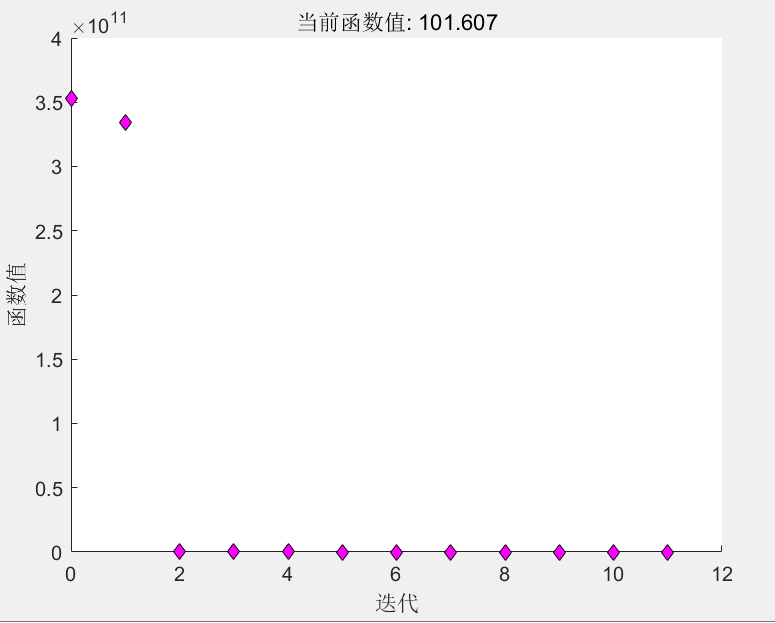
\includegraphics[width=6cm]{Optimal Control of a Linear Discrete System/MCM20200128/picture/第二问.png}
\caption{Optimization Routine}
\end{minipage}
\begin{minipage}[t]{0.48\textwidth}
\centering
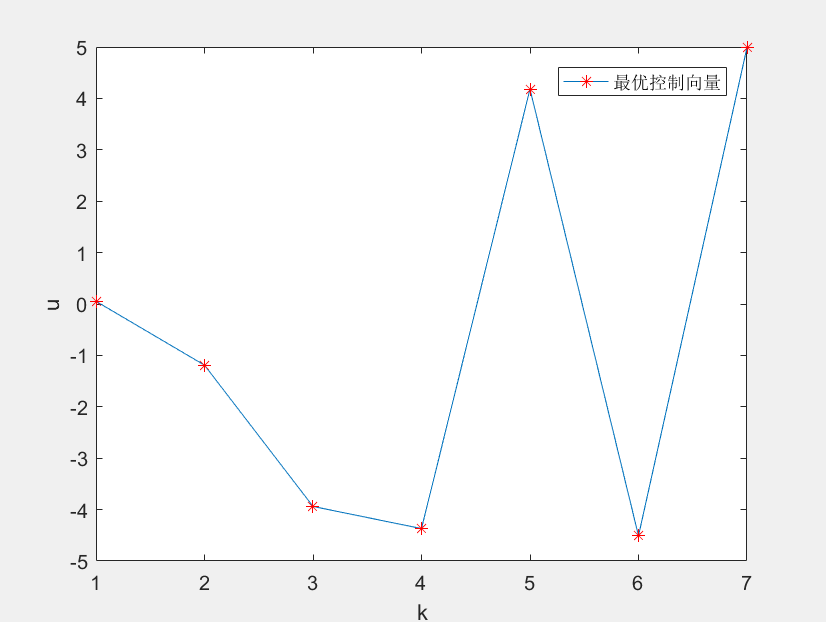
\includegraphics[width=6cm]{Optimal Control of a Linear Discrete System/MCM20200128/picture/第二问2.png}
\caption{Step of u}
\end{minipage}
\end{figure}

You can find our source code in Appendix. 

\subsection{Other methods we tried}

Along with Interior Point Method we tried a lot other methods in MATLAB, the program theories are as follows.

\subsubsection{Dynamic Programming}
The final general characteristic of the dynamic-programming approach is the development of a recursive optimization procedure, which builds to a solution of the overall N-stage problem by first solving a one-stage problem and sequentially including one stage at a time and solving one-stage problems until the overall optimum has been found. This procedure can be based on a backward induction process, where the first stage to be analyzed is the final stage of the problem and problems are solved moving back one stage at a time until all stages are included. Alternatively, the recursive procedure can be based on a forward induction process, where the first stage to be solved is the initial stage of the problem and problems are solved moving forward
one stage at a time, until all stages are included. In certain problem settings, only one of these induction processes can be applied (e.g., only backward induction is allowed in most problems involving uncertainties).

The basis of the recursive optimization procedure is the so-called principle of optimality, which has already been stated: an optimal policy has the property that, whatever the current state and decision, the remaining decisions must constitute an optimal policy with regard to the state resulting from the current decision.

Suppose we have a multistage decision process where the return (or cost) for a particular stage is:

$$f_n(d_n,s_n)$$

where dn is a permissible decision that may be chosen from the set Dn, and sn is the state of the process with n stages to go.

Noramlly, we have to solve the following problem:

\[
v_{n}\left(s_{n}\right)=\operatorname{Max}\left[f_{n}\left(d_{n}, s_{n}\right)+f_{n-1}\left(d_{n-1}, s_{n-1}\right)+\cdots+f_{0}\left(d_{0}, s_{0}\right)\right]
\]
subject to:
\[
\begin{array}{ll}
s_{m-1}=t_{m}\left(d_{m}, s_{m}\right) & (m=1,2, \ldots, n) \\
d_{m} \in D_{m} & (m=0,1, \ldots, n)
\end{array}
\]

The generally cost-to-go function is:
$$J(f, x(t))=\min _{u(t) \in U}\left\{h(x(\tau))+\int_{t}^{T} g(x(\tau) \cdot u(\tau)) d \tau\right\}$$
\subsubsection{Use DP to solve DLQR(Time limited and not use)}
The cost function in DLQR is
$$J=\sum_{n=0}^{N-1}\left(x_{n}^{T} Q x_{n}+u_{n}^{T} R u_{n}\right)+x_{N} P x_{N}$$

Where  Q,R P are positive definite matrixs.For $J_N(X_N)$ we have:
$$\begin{array}{c}
J_{N}\left(x_{N}\right)=x_{N}^{T} P x_{N} \\
J_{N-1}\left(x_{N-1}\right)=x_{N-1}^{T} Q x_{N-1}+u_{N-1}^{T} R u_{N-1}+J_{N}\left(x_{N}\right)
\end{array}$$ 

Given $x_{t+1}=A x_{k}+B_{u_{k}}$:

$$J_{N-1}\left(x_{N-1}\right)=x_{N-1}^{T} Q x_{N-1}+u_{N-1}^{T} R u_{N-1}+J_{N}\left(A x_{N-1}+B u_{N-1}\right)$$

Calculate the derivation of u and let $\nabla_{u}=0$ :

$$\begin{array}{l}
\nabla_{u}\{(2)\}=2 R u+2 B^{T} P(A x+B u)=0 \\
u=-\left(R+B^{T} P B\right)^{-1} B^{T} P A x
\end{array}$$

Sort out the upper formulas, let $u=-k x$ we can get:

$$\begin{array}{c}
J_{N-1}(x)=x^{T} \hat{P} x \\
\hat{P}=Q+k^{T} R k+(A-B k)^{T} P(A-B k)
\end{array}$$

So the DP  iterative program is:

\begin{algorithm}[H]
  \caption{Use DP solve LQR}
  \KwIn{$x_0$, A, B}
  \KwOut{$u_i$}
  \For{$i = N-1 , i>=0 , i --$}
  {
    $k=\left(R+B^{T} P B\right)^{-1} B^{T} P A$ \;
$ u_{i}=-k x $\;
$ P=Q+k^{T} R k+(A-B k)^{T} P(A-B k)$
  }
  return $(u_i)$\;
\end{algorithm}

\subsubsection{Euler Function(Hard to optimize u)}
By Lagrange undetermined multiplier method we can get:
$$\bar J=\sum^{T-1}_{k=0}\{\frac{1}{2}u^T(k)u(k)+\lambda(k+1)[-x(k+1)+Ax(k)+Bu(k)]\}$$

And this is the loss function.

Define the increment of performance indicator J in the Kth sampling period as:
$$L_k=\frac{1}{2}u^T(k)u(k)+\lambda(k+1)[-x(k+1)+Ax(k)+Bu(k)]$$

Step backward:
$$L_{k-1}=\frac{1}{2}u^T(k-1)u(k-1)+\lambda(k)[-x(k)+Ax(k-1)+Bu(k-1)]$$

Then solve the  derivation:
\begin{equation}\begin{array}{l}
\frac{\partial L_{k}}{\partial x(k)}=A^{T} \lambda^{T}(k+1) \\\\
\frac{\partial L_{k}}{\partial x(k)}=-\lambda^{T}(k) \\\\
\frac{\partial L_{k}}{\partial u(k)}=u(k)+B^{T} \lambda^{T}(k+1) \\\\
\frac{\partial L_{k}}{\partial u(k)}=0
\end{array}\end{equation}

By using Euler equation, we will have:

$$\begin{cases} A^T\lambda^T(k+1) =\lambda^T(k) \\u(k)+B^T\lambda^T(k+1)=0 \end{cases}$$

Let$\lambda^T(1)=C$, therefore:

 $$\lambda^T(k)=(A^T)^{-(k-1)}C$$

$$u(k)=-B^T(A^T)^{-k}C$$

We can easily see that

$$x(k+1)=Ax(k)-BB^T(A^T)^{-k}C$$

Thus:

\begin{align}
&x(1)=A x(0)-B B^{T} C \\
&x(2)=A^{2} x(0)-A B B^{T} C-B B^{T}\left(A^{T}\right)^{-1} C \\
&x(3)=A^{3} x(0)-A^{2} B B^{T} C-A B B^{T}\left(A^{T}\right)^{-1} C-B B^{T}\left(A^{T}\right)^{-2} C \\
\cdots \\
& x(k+1)=A^{k+1} x(0)-\sum_{i=0}^{k} A^{k-i} B B^{T}\left(A^{T}\right)^{-i} C
\end{align}

So Euler Function constrains u into a small  feasible region and we can solve it by iteration methods.

Unfortunately, this method cannot set u's limitation, it can only get the globally optimal solution, but we think this method works in optimize the cost function.

%%%%%%%%%%%%%%%%%%%%%%%%%%%%%%
%%%%%%%%%%%%%%%%%%%%%%%%%%%%%%%
%%%%%%%%%%%%%%%%%%%%%%%%%%%%
%%%%%%%%%%%%%%%%%%%%%%%%%%%%%%%%%%%%%%%%%%%%%%%%%%%%%%

\section{Problem Three: Change A and analyze its impact}
According to the gain K that we have calculated earlier, we inferred that the increase of A may lead to the raise of control series. After making trail of this method, we obtained the following experiment results which gave a visual representation of our inference.\cite{MatthewGSmith:2005:GPEM}\cite{conf/smc/NetoFR13}

Our code for interior point method is:

\begin{lstlisting}[language=MATLAB, caption=Function for interior point method]
function y = fitness(u)
[rows,cols]=size(u);
x= [0.05; 0.08; 0]
A=[100 0 0;0 100 0;0 0 100];
B=[2;1;1];
sum=0;
L = 2
for k=1:1:cols
    x=A*x+B*u(k);
end
for k=2:1:cols
    sum=sum+u(k) * u(k);
end
y= sum + L * (x'*x);
end
\end{lstlisting}

Which defines the function for optimizer. And we will change A for experiment.

%%制作3*3子图
\begin{figure}[H]
\centering
\subfigure[\text{A = diag(1 1 1)}]{
\begin{minipage}[t]{27ex}
\centering
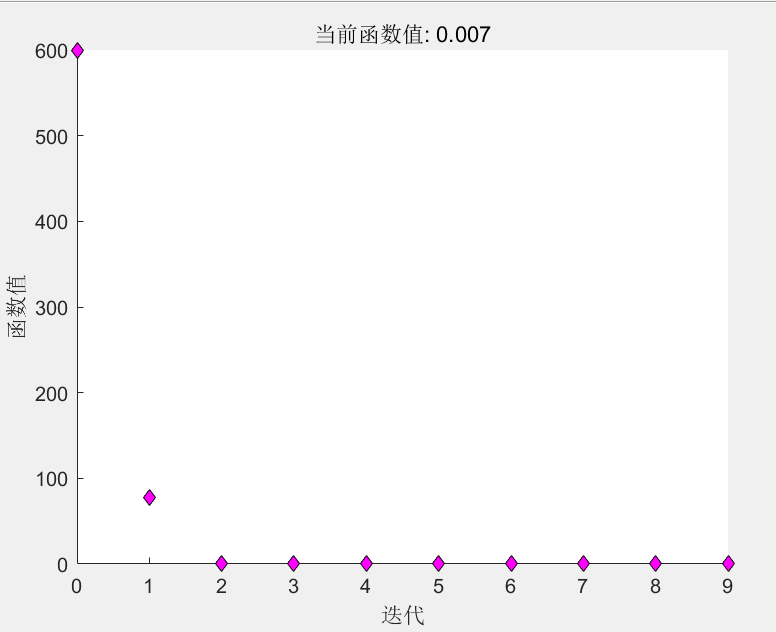
\includegraphics[width=26ex]{Optimal Control of a Linear Discrete System/MCM20200128/picture/changeA/图片1.png}
%\caption{fig1}
\end{minipage}%
}%
\subfigure[\text{A = diag(10 10 10)}]{
\begin{minipage}[t]{27ex}
\centering
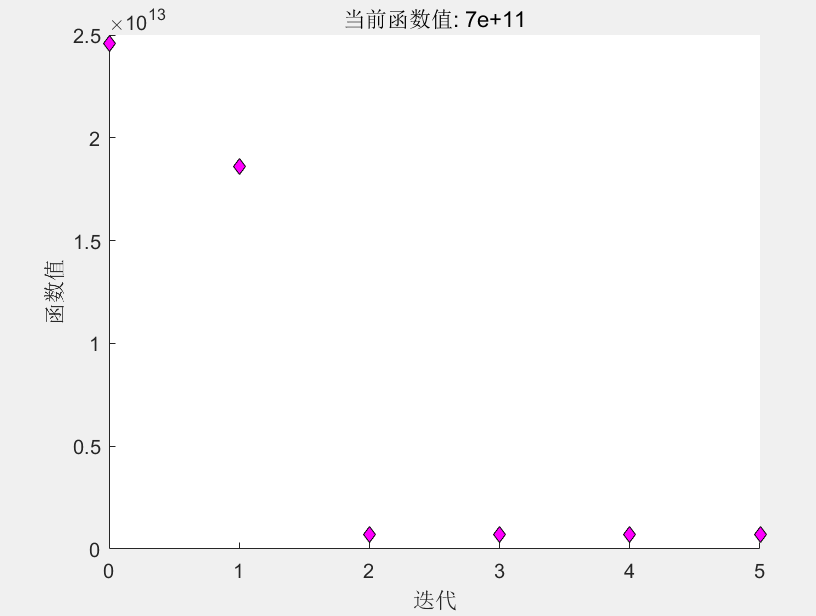
\includegraphics[width=26ex]{Optimal Control of a Linear Discrete System/MCM20200128/picture/changeA/图片2.png}
%\caption{fig2}
\end{minipage}%
}%
\subfigure[\text{A=diag(20 20 20)}]{
\begin{minipage}[t]{27ex}%0.4行往后
\centering
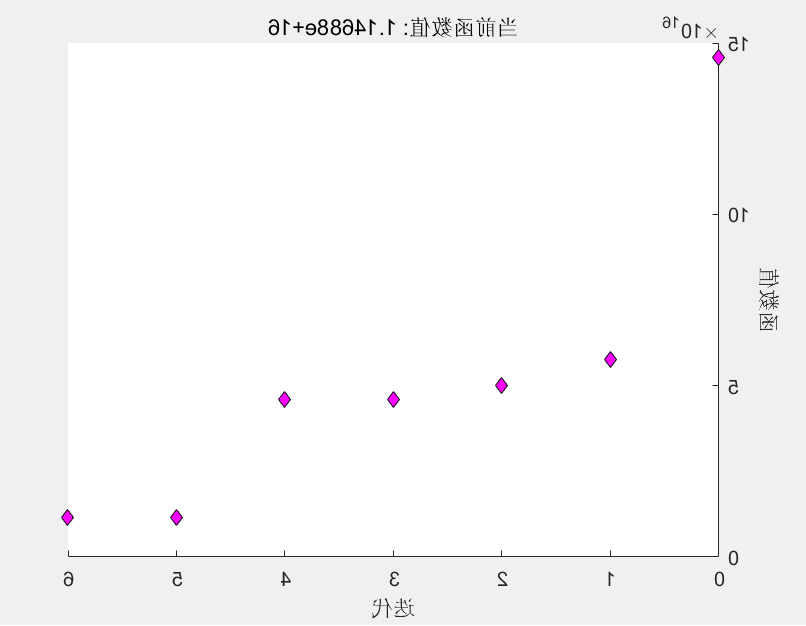
\includegraphics[width=26ex]{Optimal Control of a Linear Discrete System/MCM20200128/picture/changeA/图片3.png}
%\caption{fig2}
\end{minipage}%
}%

                 %这个回车键很重要 \quad也可以,代表换行
\subfigure[\text{A = diag(30 30 30)}]{
\begin{minipage}[t]{27ex}
\centering
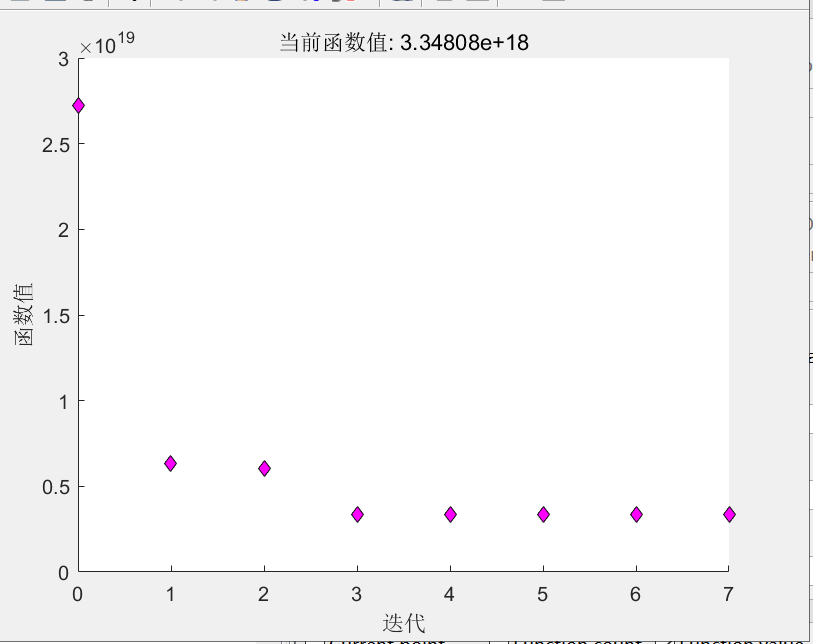
\includegraphics[width=26ex]{Optimal Control of a Linear Discrete System/MCM20200128/picture/changeA/图片4.png}
%\caption{fig2}
\end{minipage}
}%
\subfigure[\text{A = diag(50 50 50)}]{
\begin{minipage}[t]{27ex}
\centering
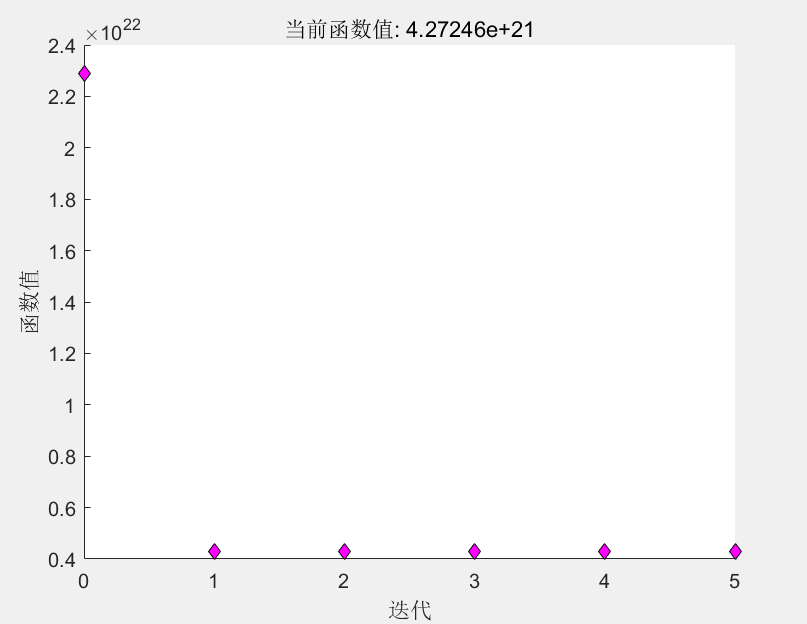
\includegraphics[width=26ex]{Optimal Control of a Linear Discrete System/MCM20200128/picture/changeA/图片5.png}
%\caption{fig2}
\end{minipage}
}%
\subfigure[\text{A = diag(70 70 70)}]{
\begin{minipage}[t]{27ex}
\centering
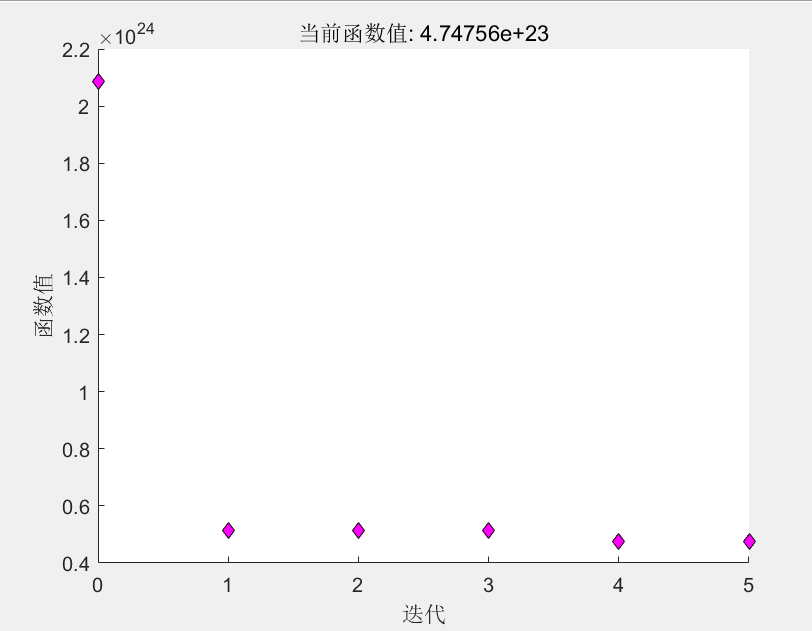
\includegraphics[width=26ex]{Optimal Control of a Linear Discrete System/MCM20200128/picture/changeA/图片6.png}
%\caption{fig2}
\end{minipage}
}%

                 %这个回车键很重要 \quad也可以,代表换行
\subfigure[\text{A = diag(100 100 100)}]{
\begin{minipage}[t]{27ex}
\centering
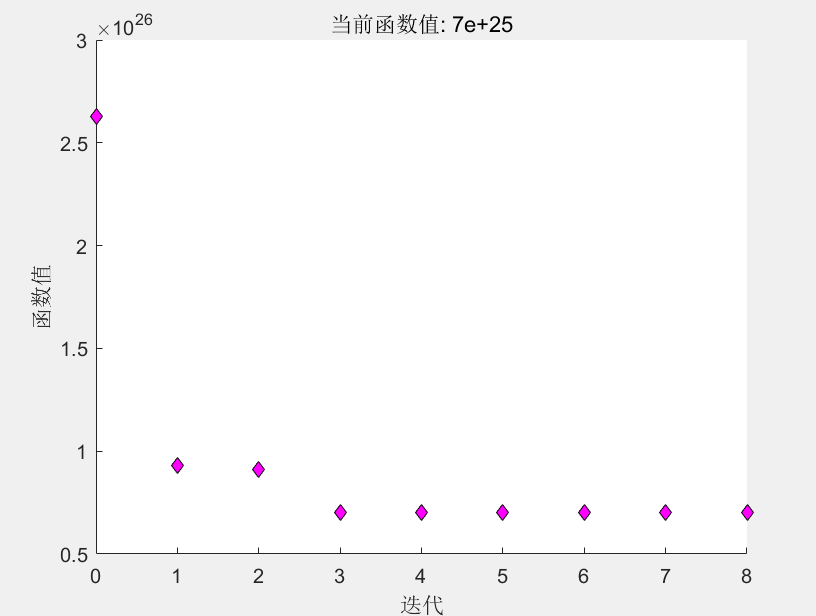
\includegraphics[width=26ex]{Optimal Control of a Linear Discrete System/MCM20200128/picture/changeA/图片7.png}
%\caption{fig2}
\end{minipage}
}%
\subfigure[\text{A = diag(500 500 500)}]{
\begin{minipage}[t]{27ex}
\centering
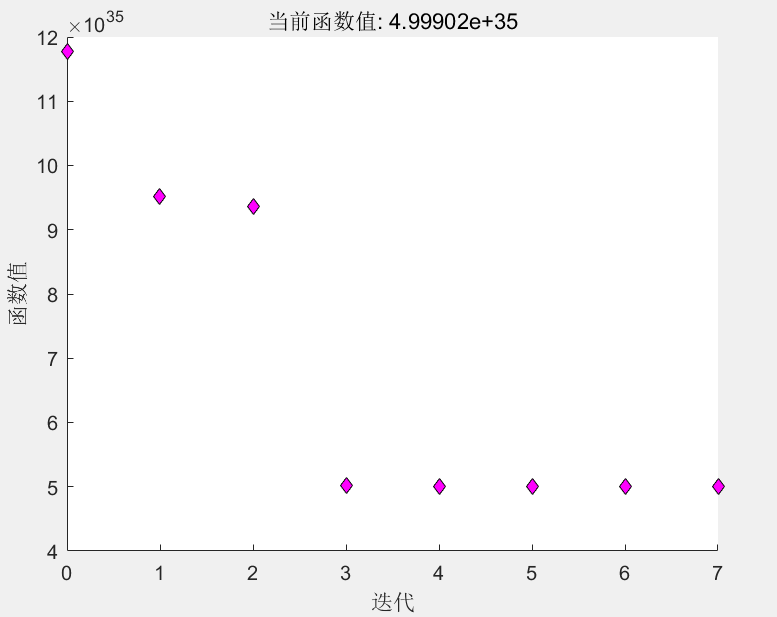
\includegraphics[width=26ex]{Optimal Control of a Linear Discrete System/MCM20200128/picture/changeA/图片8.png}
%\caption{fig2}
\end{minipage}
}%
\subfigure[\text{A = diag(1000 1000 1000)}]{
\begin{minipage}[t]{27ex}
\centering
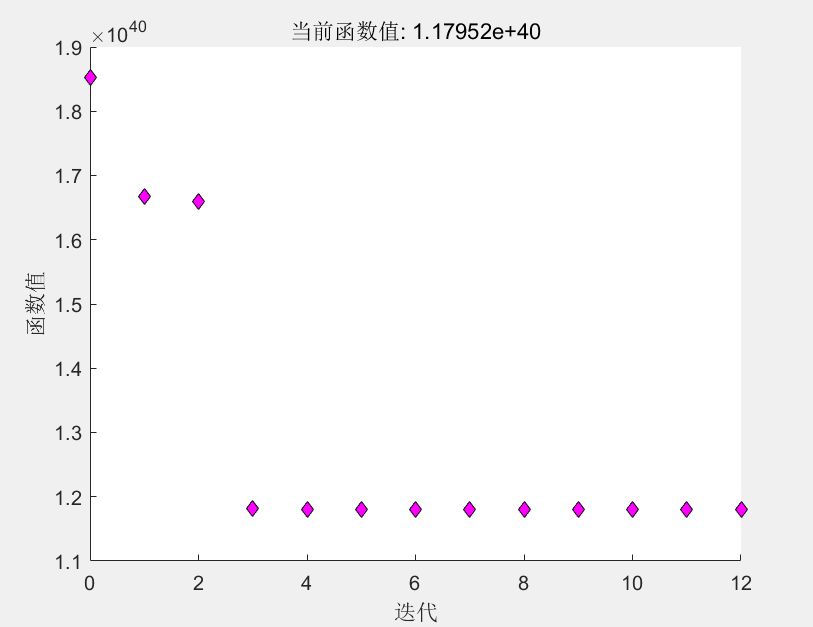
\includegraphics[width=26ex]{Optimal Control of a Linear Discrete System/MCM20200128/picture/changeA/图片9.png}
%\caption{fig2}
\end{minipage}
}%


\centering
\caption{Step of x while changing value of A}
\end{figure}


From the screenshots, we can see that the value of controls indeed increase with the growth of A at the beginning. Intuitively, we can see that when A is relatively large, the whole system will need to have a much bigger negative feedback at the beginning in order to constrain the state x(T) at the end to fall in a predetermined interval. After the x(t) is small enough, we only need small controls to adjust the system. If the controls are not big enough at the beginning, the x(t) will grow to a much larger number which may cause even bigger controls. Therefore the objective function will be able to reach the optimal value.

\begin{figure}[H]%H为当前位置,!htb为忽略美学标准,htbp为浮动图形
  \centering
  \caption{Steps of u}
%可选参数中width=\columnwidth选取了当前列宽
  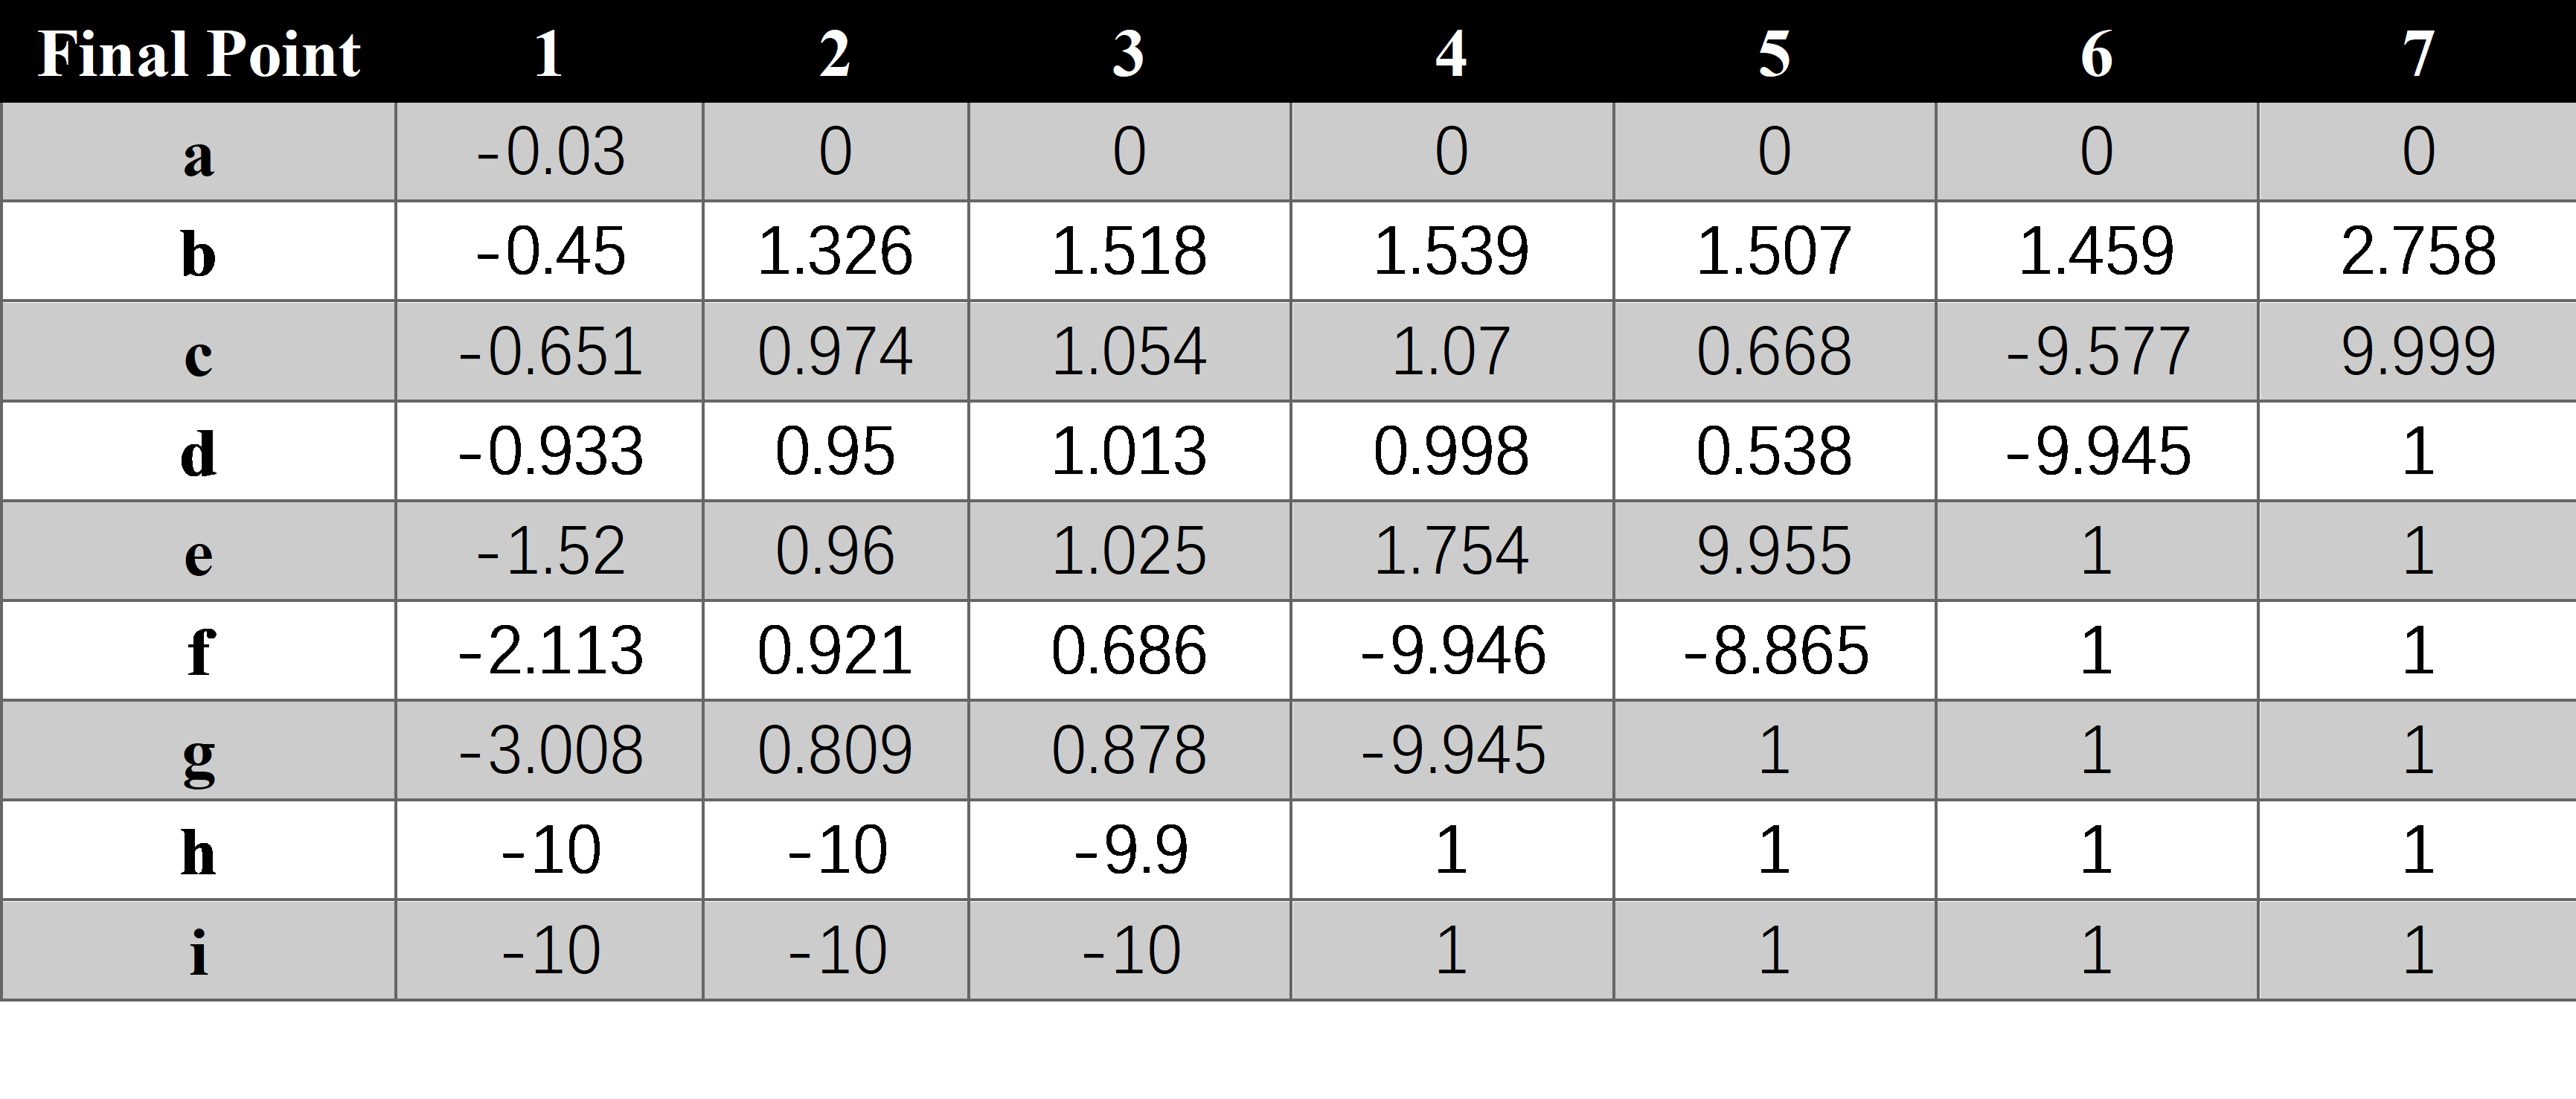
\includegraphics[width=50ex]{Optimal Control of a Linear Discrete System/MCM20200128/picture/changeA/表格.png} %插入图片,[]中设置图片大小,{}中是图片文件名
  \label{Fig.RNN} %用于文内引用的标签
\end{figure}


\section{Problem Four: Change upper bounds}
When we change the upper bounds, it can be seen from the screenshots that when the upper bound becomes smaller, the value of the objective function will become smaller. At the same time, the values of a few controls become closer to the upper bound. Obviously, when the upper bound becomes smaller, the x(T) becomes more difficult or even impossible to fall into the given range.
\begin{figure}[H]
\centering

\subfigure[T= 7  upper = 5   low=-5]{
\begin{minipage}[t]{25ex}
\centering
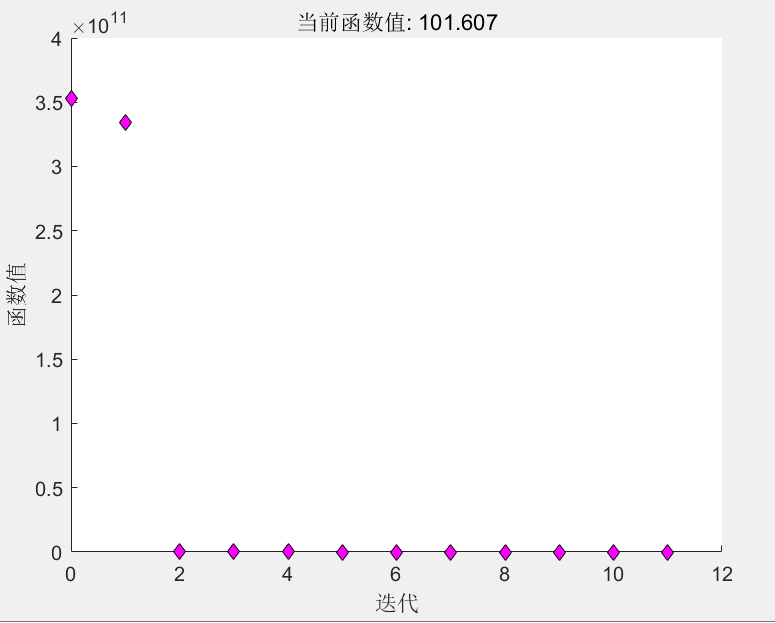
\includegraphics[width=22ex]{Optimal Control of a Linear Discrete System/MCM20200128/picture/第二问.png}
%\caption{fig1}
\end{minipage}%
}%
\subfigure[T= 7  upper = 5   low=-5]{
\begin{minipage}[t]{25ex}
\centering
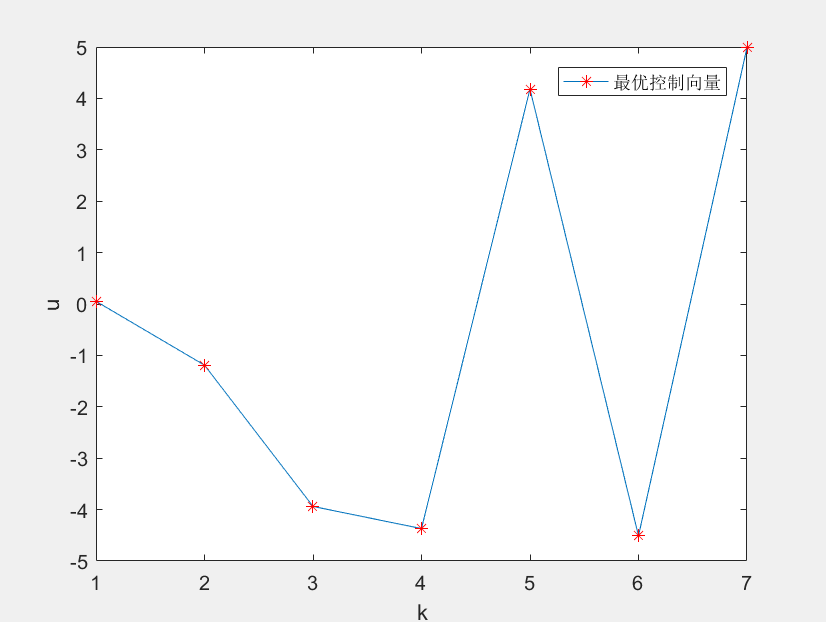
\includegraphics[width=22ex]{Optimal Control of a Linear Discrete System/MCM20200128/picture/第二问2.png}
%\caption{fig2}
\end{minipage}%
}%

                 %这个回车键很重要 \quad也可以
\subfigure[T= 7  upper = 2   low=-2]{
\begin{minipage}[t]{25ex}
\centering
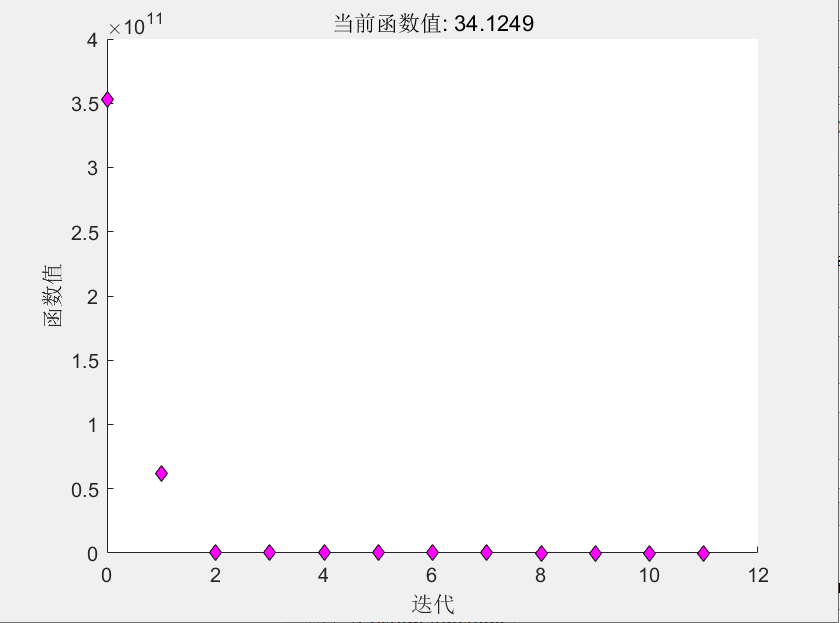
\includegraphics[width=22ex]{Optimal Control of a Linear Discrete System/MCM20200128/picture/CB/CB1.png}
%\caption{fig2}
\end{minipage}
}%
\subfigure[T= 7  upper = 2   low=-2]{
\begin{minipage}[t]{25ex}
\centering
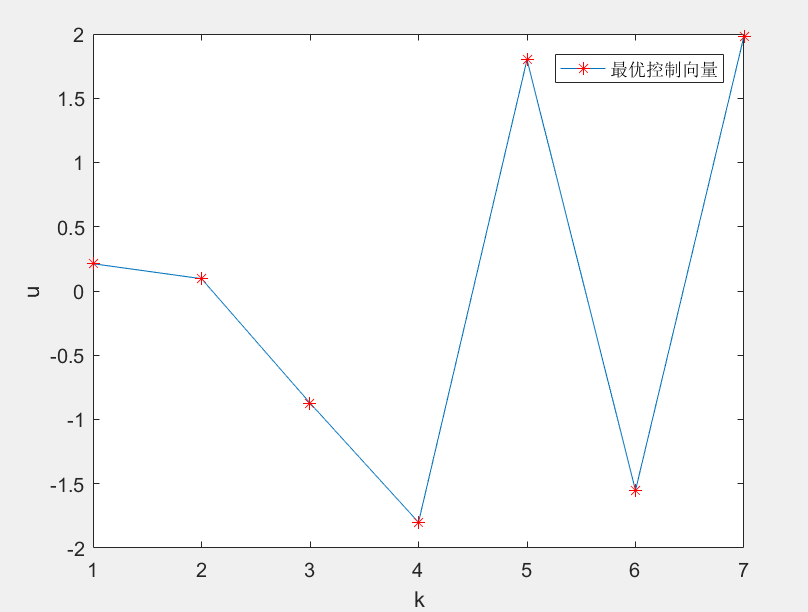
\includegraphics[width=22ex]{Optimal Control of a Linear Discrete System/MCM20200128/picture/CB/CB2.png}
%\caption{fig2}
\end{minipage}
}%

                 %这个回车键很重要 \quad也可以
\subfigure[T= 7  upper = 10   low=-10]{
\begin{minipage}[t]{25ex}
\centering
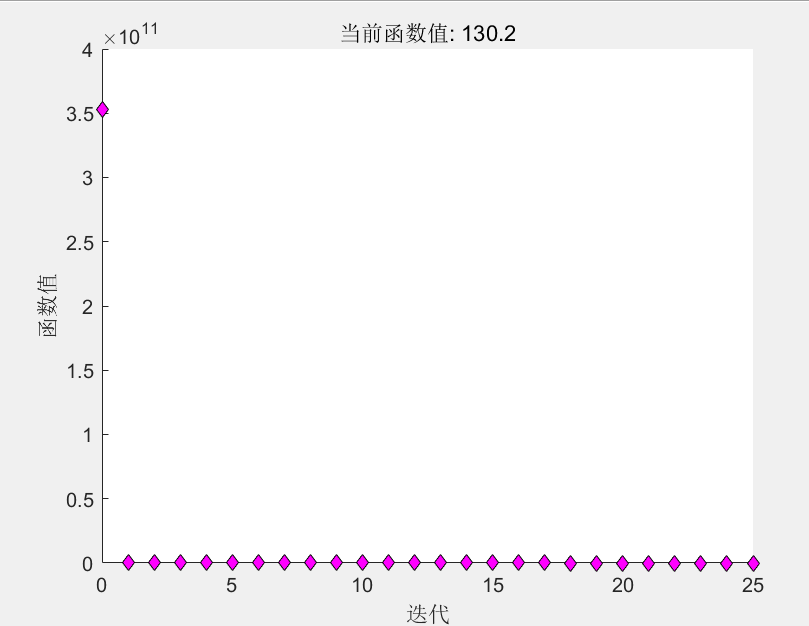
\includegraphics[width=22ex]{Optimal Control of a Linear Discrete System/MCM20200128/picture/CB/CB3.png}
%\caption{fig2}
\end{minipage}
}%
\subfigure[T= 7  upper = 10   low=-10]{
\begin{minipage}[t]{25ex}
\centering
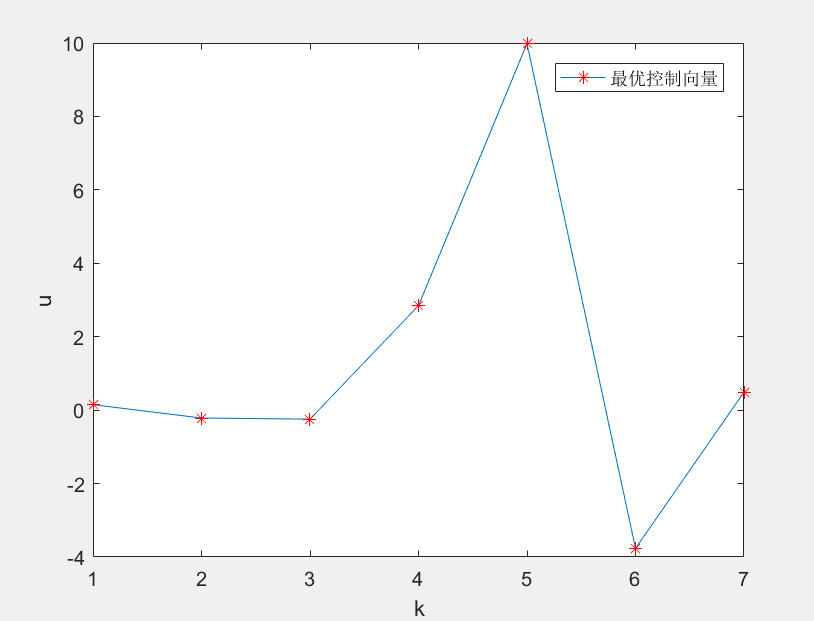
\includegraphics[width=22ex]{Optimal Control of a Linear Discrete System/MCM20200128/picture/CB/CB4.png}
%\caption{fig2}
\end{minipage}
}%
\centering
\caption{Change the bounds }
\end{figure}


\section{Problem Five: Change  the length of the time horizon: T}

The screenshots show that when the T becomes larger, the value of the objective function will become sharply larger. When the T becomes super large, the values of the last few controls become close to the same value.


\begin{figure}[H]
\centering

\subfigure[T= 7  upper = 5   low=-5]{
\begin{minipage}[t]{25ex}
\centering
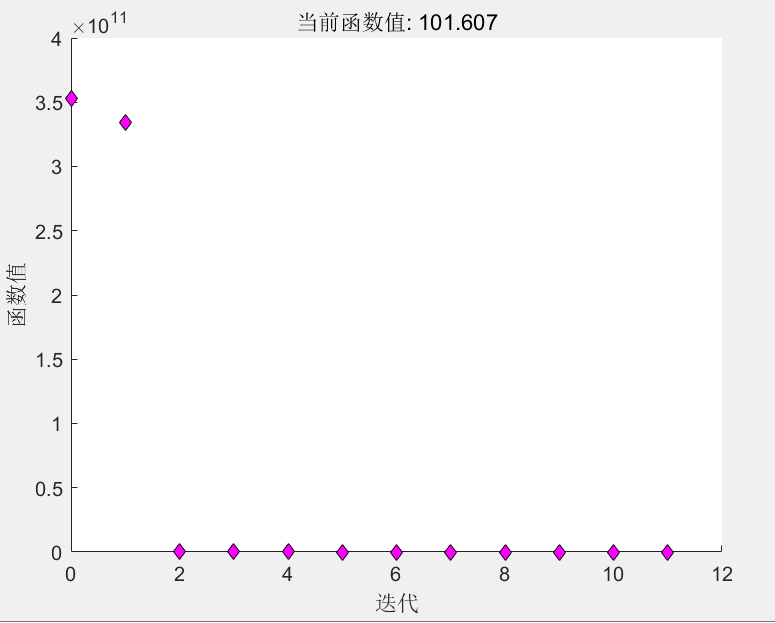
\includegraphics[width=22ex]{Optimal Control of a Linear Discrete System/MCM20200128/picture/第二问.png}
%\caption{fig1}
\end{minipage}%
}%
\subfigure[T= 7  upper = 5   low=-5]{
\begin{minipage}[t]{25ex}
\centering
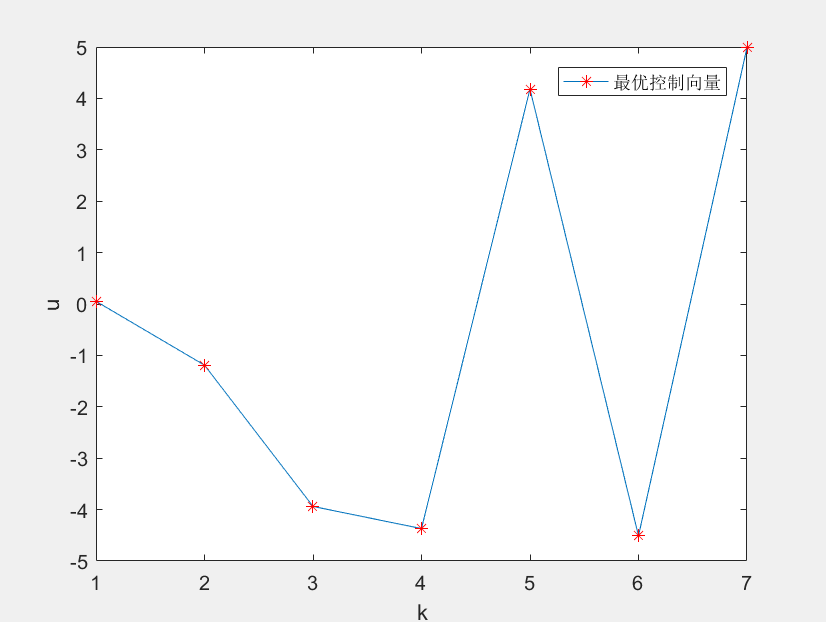
\includegraphics[width=22ex]{Optimal Control of a Linear Discrete System/MCM20200128/picture/第二问2.png}
%\caption{fig2}
\end{minipage}%
}%

                 %这个回车键很重要 \quad也可以
\subfigure[T= 5  upper = 5   low=-5]{
\begin{minipage}[t]{25ex}
\centering
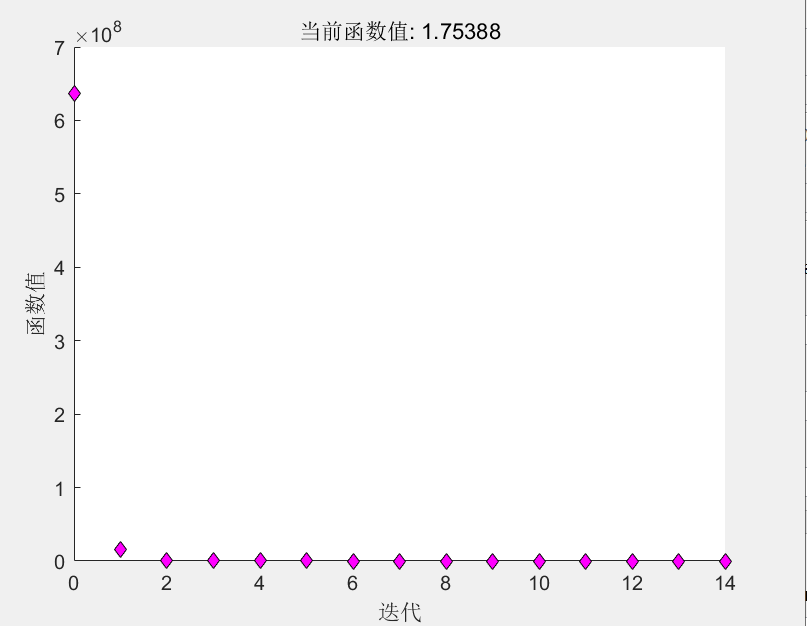
\includegraphics[width=22ex]{Optimal Control of a Linear Discrete System/MCM20200128/picture/CT/CT1.png}
%\caption{fig2}
\end{minipage}
}%
\subfigure[T= 5  upper = 5   low=-5]{
\begin{minipage}[t]{25ex}
\centering
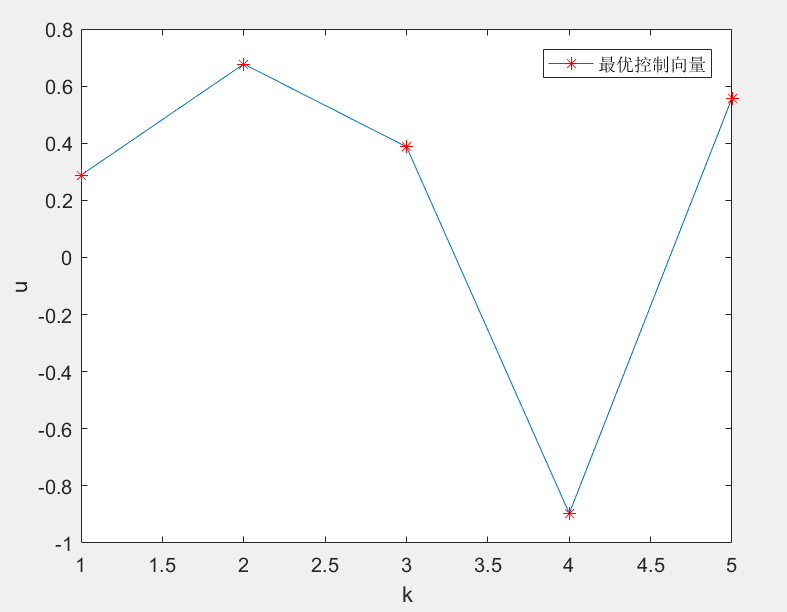
\includegraphics[width=22ex]{Optimal Control of a Linear Discrete System/MCM20200128/picture/CT/CT2.png}
%\caption{fig2}
\end{minipage}
}%

                 %这个回车键很重要 \quad也可以
\subfigure[T= 10  upper = 5   low=-5]{
\begin{minipage}[t]{25ex}
\centering
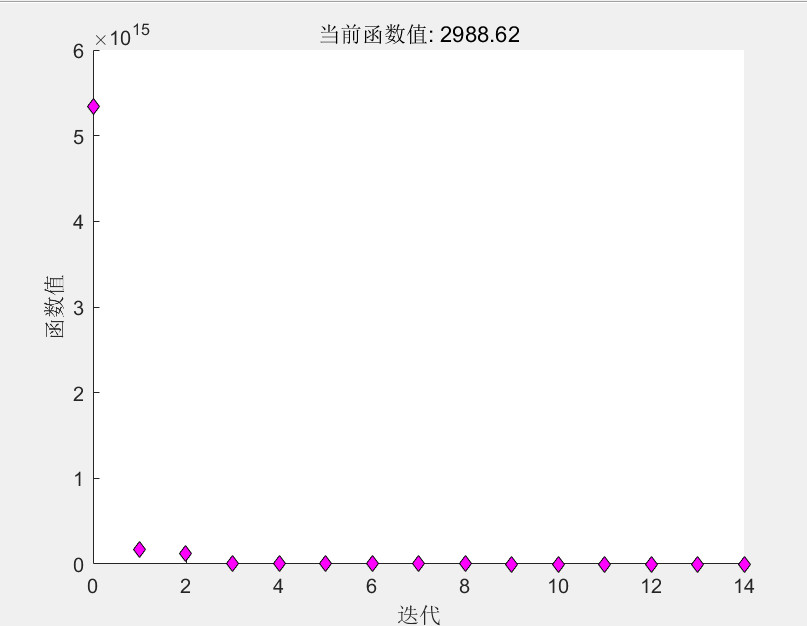
\includegraphics[width=22ex]{Optimal Control of a Linear Discrete System/MCM20200128/picture/CT/CT3.png}
%\caption{fig2}
\end{minipage}
}%
\subfigure[T= 7  upper = 10   low=-10]{
\begin{minipage}[t]{25ex}
\centering
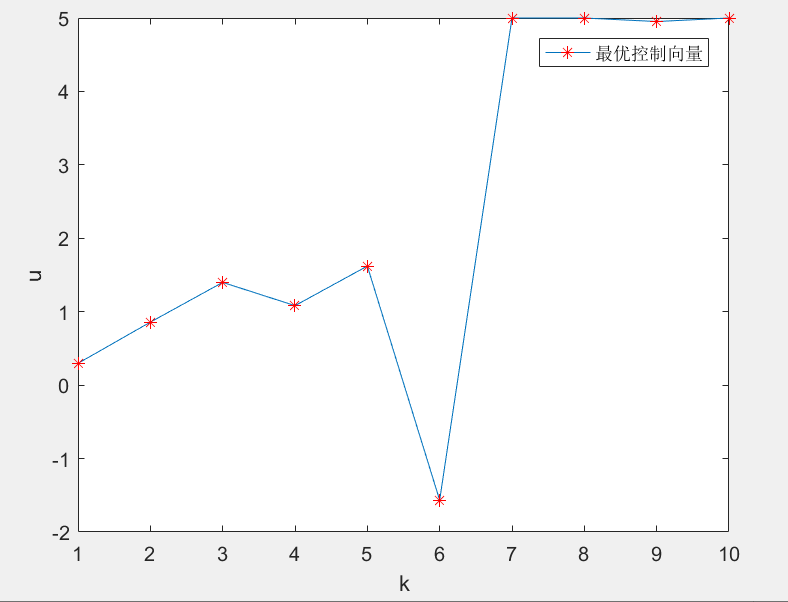
\includegraphics[width=22ex]{Optimal Control of a Linear Discrete System/MCM20200128/picture/CT/CT4.png}
%\caption{fig2}
\end{minipage}
}%
\centering
\caption{Change the length of the time horizon}
\end{figure}


\addcontentsline{toc}{section}{Reference}
\bibliographystyle{plain}
\bibliography{myreference}

\begin{appendices}

\section{ Source Code}
\begin{itemize}
\item Code in MATLAB for DLQR:
\end{itemize}
\begin{lstlisting}[language=MATLAB, caption=LQR in MATLAB]
A=[0 1 0;0 0 1;-35 -27 -9];
B=[0;0;1];
C=[1 0 0 ;0 1 0 ;0 0 1 ];
D=[0;0;0;];
Q=[0 0 0;0 0 0;0 0 0];
R=1;
K=dlqr(A,B,Q,R)
Ac=[(A-B*K)];
Bc=[B];
Cc=[C];
Dc=[D];
t=0:0.005:200;
U=ones(size(t));
x0=[0.05 0.08 0];
[Y,X]=lsim(Ac,Bc,Cc,Dc,U,t,x0);
plot(t,Y);
xlabel('t');
ylabel('Y');
u=-K*X';
\end{lstlisting}
\begin{itemize}
\item Code in MATLAB for interior point method:
\end{itemize}

\begin{lstlisting}[language=MATLAB, caption=Function for interior point method]
function y = fitness(u)
[rows,cols]=size(u);
x= [0.05; 0.08; 0]
A=[100 0 0;0 100 0;0 0 100];
B=[2;1;1];
sum=0;
L = 2
for k=1:1:cols
    x=A*x+B*u(k);
end
for k=2:1:cols
    sum=sum+u(k) * u(k);
end
y= sum + L * (x'*x);
end
\end{lstlisting}


\end{appendices}
\end{document}
